\section{Task 2}

\subsection{Overview of Neville's algorithm}

Neville's algorithm evaluates an interpolating polynomial at a given point. It efficiently evaluates polynomials from a specified set of points, although its \( O(n^2) \) complexity can be costly for large datasets.

Neville interpolation uses a recurrence to compute the function value at \( x \) from points \( (x_i, y_i) \). Tests sampled \( n \) points from \( D = (0, 10) \), then compared interpolated and actual function values at 100 evenly spaced points.

Four functions were tested:
\begin{itemize}
    \item Trigonometric function: \( f(x) = \sin(x) + \cos(x) \),
    \item Degree-3 polynomial: \( f(x) = x^3 - 2x + 1 \),
    \item Exponential function: \( f(x) = e^x \),
    \item Rational function: \( f(x) = \frac{1}{1 + x^2} \).
\end{itemize}

For each function, the interpolation error, its standard deviation and the algorithm runtime were computed.

\subsection{Results and conclusions}

\begin{center}
\textbf{Trigonometric-function results:}
Minimum error: \( 2.01 \times 10^{-13} \pm 1.03 \times 10^{-12} \), at 23 points.

\begin{minipage}{0.49\textwidth}
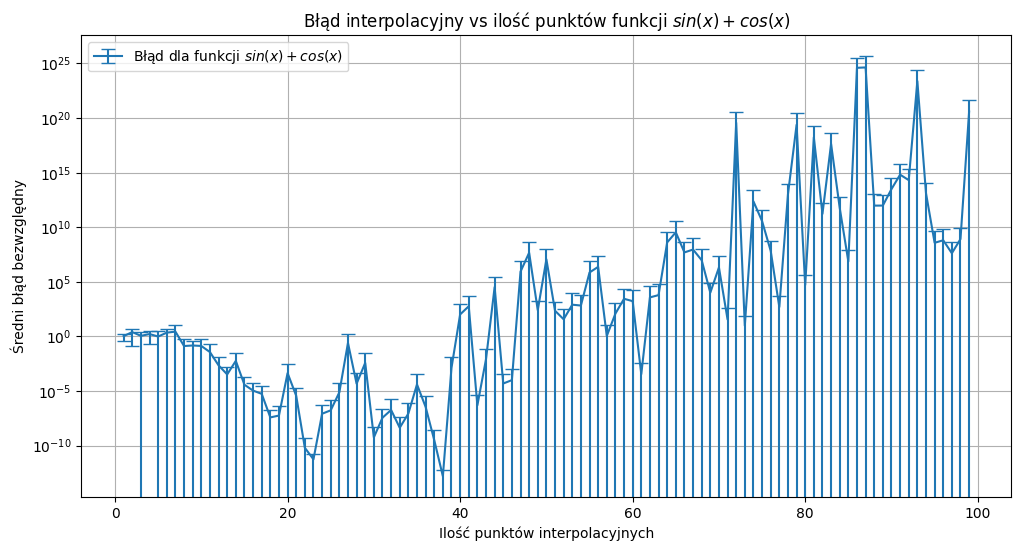
\includegraphics[width=\textwidth]{figures/task-2/error_trigonometric.png}
\end{minipage}
\begin{minipage}{0.49\textwidth}
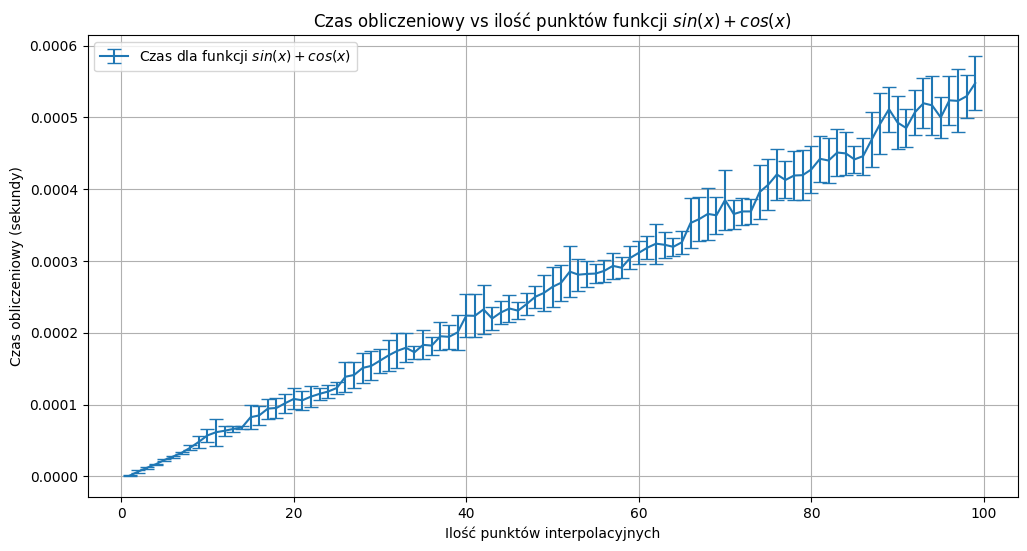
\includegraphics[width=\textwidth]{figures/task-2/runtime_trigonometric.png}
\end{minipage}

\textbf{Degree-3 polynomial results:}
Minimum error: \( 8.21 \times 10^{-14} \pm 1.31 \times 10^{-13} \),
at 9 points.

\begin{minipage}{0.49\textwidth}
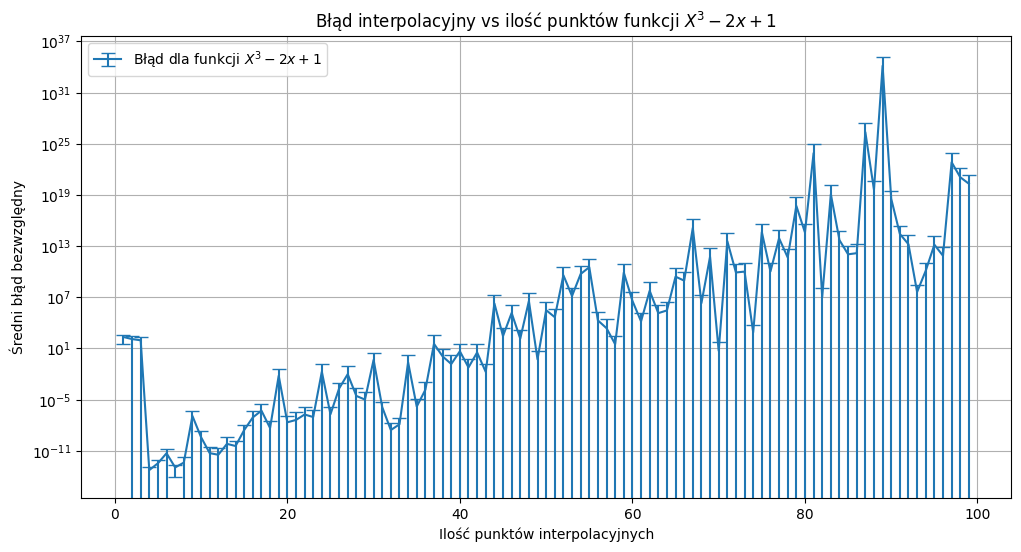
\includegraphics[width=\textwidth]{figures/task-2/error_polynomial.png}
\end{minipage}
\begin{minipage}{0.49\textwidth}
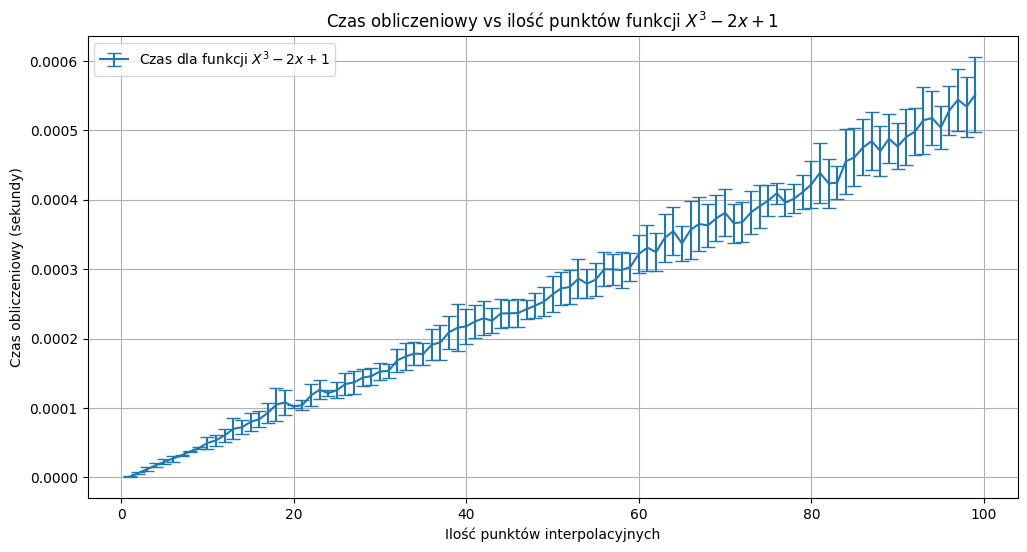
\includegraphics[width=\textwidth]{figures/task-2/runtime_polynomial.png}
\end{minipage}

\textbf{Exponential-function results:}
Minimum error: \( 2.00 \times 10^{-9} \pm 1.25 \times 10^{-8} \),
at 26 points.

\begin{minipage}{0.49\textwidth}
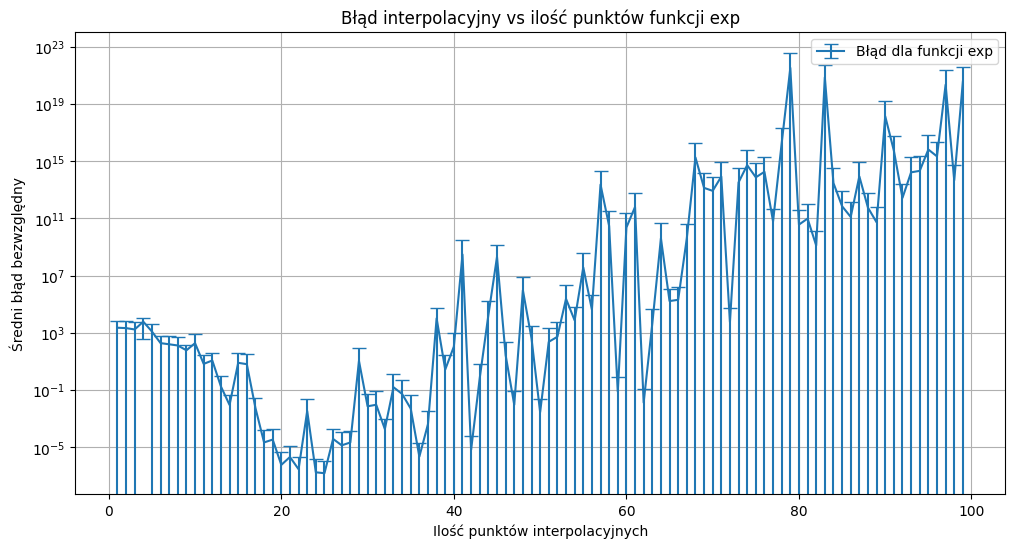
\includegraphics[width=\textwidth]{figures/task-2/error_exp.png}
\end{minipage}
\begin{minipage}{0.49\textwidth}
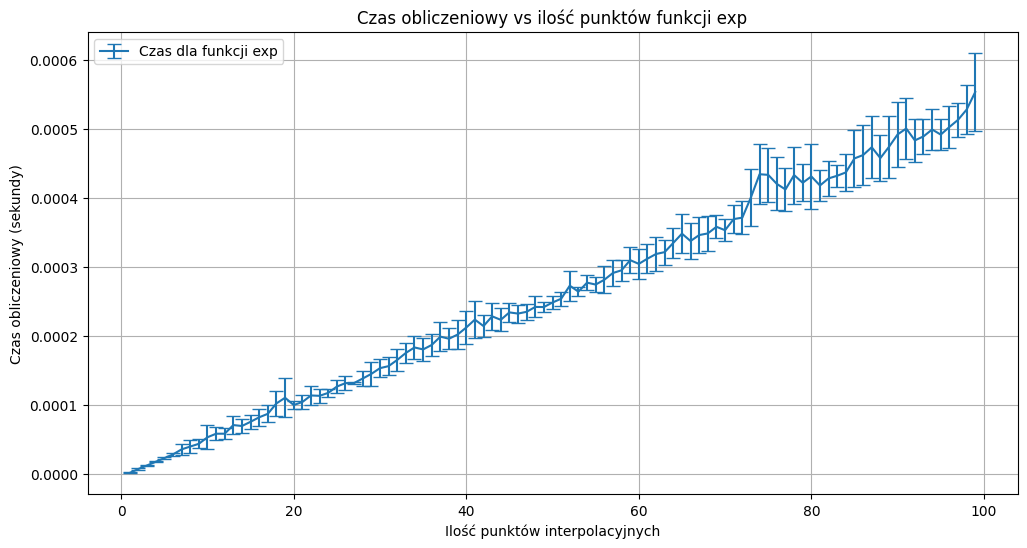
\includegraphics[width=\textwidth]{figures/task-2/runtime_exp.png}
\end{minipage}

\textbf{Results for $\frac{1}{1 + x^2}$:}
Minimum error: \( 7.63 \times 10^{-12} \pm 3.28 \times 10^{-11} \),
at 28 points.

\begin{minipage}{0.49\textwidth}
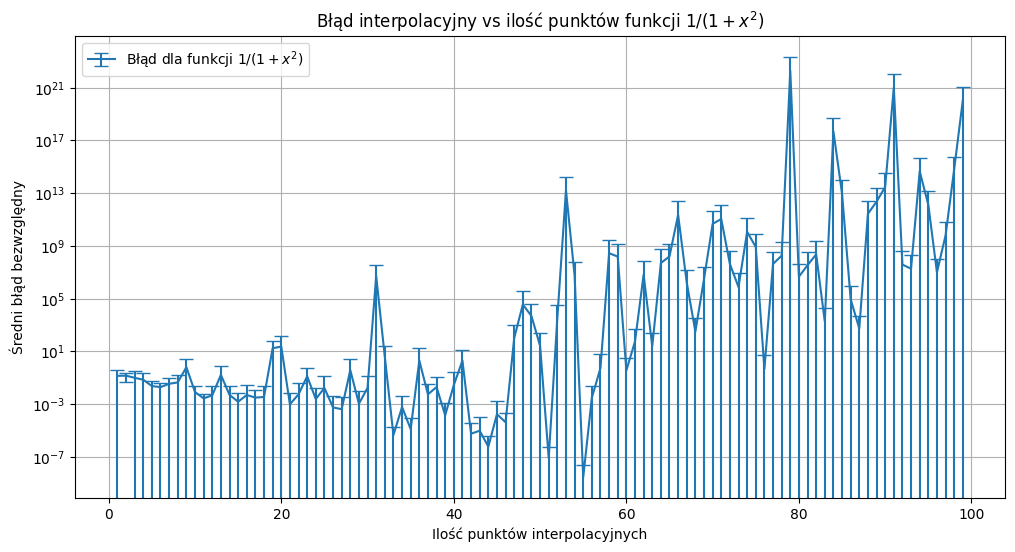
\includegraphics[width=\textwidth]{figures/task-2/error_rational.png}
\end{minipage}
\begin{minipage}{0.49\textwidth}
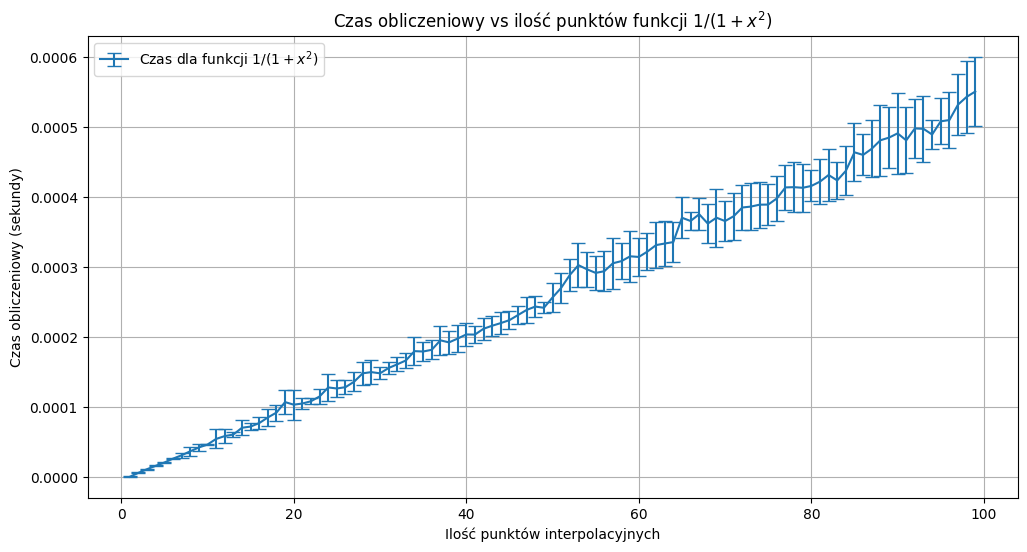
\includegraphics[width=\textwidth]{figures/task-2/runtime_rational.png}
\end{minipage}
\end{center}

\textbf{Conclusions:}
\begin{itemize}
    \item \textbf{Precision for 10--20 points:} Using 10 to 20 points gave the best accuracy. More points increased errors, mainly through numerical effects from large increments. However, the standard deviation was large.
    \item \textbf{Computation time:} Neville's runtime was linear in the number of points, with a very small growth coefficient. This follows from the implementation.
    \item \textbf{Differences between functions:} The exponential function gave the largest errors because of its rapid growth over \( D \). The cubic polynomial gave the smallest errors, as expected because polynomial interpolation is ideal for this function type.
    \item \textbf{Standard deviation and error:} The unusual display of standard deviation is caused by plot rescaling. It mainly indicates whether the deviation rises substantially.
\end{itemize}
